% == Worksheet 4
%\newpage
%~
\newpage
\stepcounter{handout}
\begin{exercisebox}[adjusted title= Animation and Functions]% \ttpy{setup}/\ttpy{draw}]

Please create a new temporary project (you don't need to save it). Type in
this piece of code:

\begin{lstlisting}[language=JavaScript]
// declare global variable accessible from any part of the code
let globalVarX = 50;

function setup() {
  createCanvas(400, 400);
}

function draw() {
  background(220);
  background(255, 255, 255);
  fill(255, 0, 0);
  ellipse(globalVarX, 100, 30, 30);
  globalVarX = globalVarX + 1;
}

\end{lstlisting}

\noindent
The \ttpy{draw} function is automatically called 60 times per second!

\tcbsubtitle{Tasks:}
\begin{itemize}
\item Try changing  $50$ in \ttpy{globalVarX} to different number.
\item Try changing the line \ttpy{x = x + 1} to \ttpy{x = x - 1} or to \ttpy{x = x + 5}
\item Try moving the call to \ttpy{background} from \ttpy{draw}
  to \ttpy{setup} - what happens?
\end{itemize}


\tcbsubtitle{NOTE!!:}  % check this
When using
\ttpy{setup}/\ttpy{draw}~ it is not allowed to call
drawing functions outside of \ttpy{setup} and
\ttpy{draw}, everything must be moved into the two functions.

\end{exercisebox}

\begin{exercisebox}[adjusted title= Aquarium continues]
\begin{itemize}
\item \emph{Rewriting the aquarium project to use \ttpy{setup}/\ttpy{draw}:}
 \begin{itemize}
 \item Add empty \ttpy{setup} and \ttpy{draw} functions to the bottom of the program
 \item Call \ttpy{size(400, 400)} in \ttpy{setup}
 \item Call all the drawing functions in \ttpy{draw}, incl. drawing of the background
 \end{itemize}

\item \emph{Make the fish swim:}
 \begin{itemize}
 \item Create two global variables \ttpy{fish1X} and
 \ttpy{fish2X} (before \ttpy{setup}/\ttpy{draw})
 \item Use the new variables as x-argument when you call \ttpy{drawFish()}
 \item \emph{REMEMBER} the lines: ~\ttpy{global fish1X}~ and ~\ttpy{global fish2X}~
 \item Update the variables with $+1$/$-1$ inside the \ttpy{draw} function
 \end{itemize}
\end{itemize}
\end{exercisebox}

\begin{exercisebox}[adjusted title= Green City continues]

\begin{itemize}
\item Create two global variables \ttpy{carX} and \ttpy{cloudX}
\item Make the car drive to the right
\item Make the cloud start outside the image on the right side and move to the left
\end{itemize}
\end{exercisebox}


%%\emph{TODO: illustrationer}
\begin{exercisebox}[adjusted title= Randomness]
Create a brand new project and save it as ``random\_circles''. Add the following code:
\begin{minipage}{0.60\linewidth}

\begin{lstlisting}[language=JavaScript]
function setup() {
  createCanvas(400, 400);
  background(220);
}

function draw() {
  // create 2 variables for different x y coordinates on the canvas
  let x = random(0, width);
  let y = random(0, height);
  
  // color the circle with a random monochrome shade
  fill(random(255));
  
  // draw the ellipse every frame
  ellipse(x, y, 30, 30);
}

\end{lstlisting}
\end{minipage}

\begin{minipage}{0.40\linewidth}
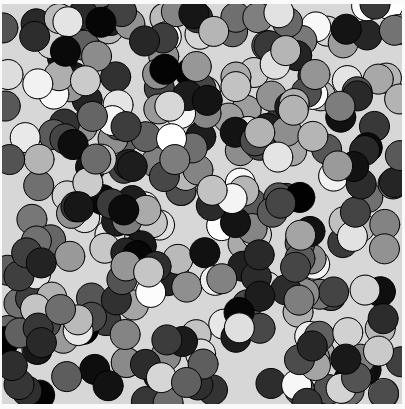
\includegraphics[width=0.70\textwidth]{illustrationer/randomcircles.png}
\end{minipage}
~
\end{exercisebox}

%\begin{minipage}{0.45\textwidth}
%\begin{Right}

%\end{Right} \end{minipage}

\begin{exercisebox}[adjusted title=Tasks: ]


\begin{itemize}
\item Make the circles change size randomly
\item Make the circles be drawn in random colours. Experiment until you find a colour scale that you think is nice.
\end{itemize}

\end{exercisebox}

\begin{exercisebox}[adjusted title=Interaction with the Mouse]
The position of the mouse can be read with the variables \ttpy{mouseX}
and \ttpy{mouseY}. A kind of drawing program can be written like this:

\begin{lstlisting}[language=JavaScript]
function setup() {
  createCanvas(800, 800);
  background(255, 204, 0);
}

function draw() {
  fill(0, 0, 0);
  ellipse(mouseX, mouseY, 5, 5);
}

\end{lstlisting}

\end{exercisebox}

\begin{exercisebox}[adjusted title=Keyboard input]
%\chapter{Tastatur input}
Åbn tegneprograms-projektet og prøv at tilføje følgende nye funktion:

\begin{lstlisting}[language=JavaScript]
function setup() {
  createCanvas(400, 400);
  background(0);
}

function draw() {
  
}

function keyPressed(){
  background(0,0,255,255);
}
\end{lstlisting}

Start the program and press any key on the keyboard. To
check for a specific key, the variable ``\ttpy{key}'' can be read.

\begin{lstlisting}[language=JavaScript]
 if (key == 'c') { // Check if the 'c' key is pressed
    background(255, 204, 0); // Set background color to a blue hue
\end{lstlisting}
%NEED FOOTNOTE
\end{exercisebox}

\begin{exercisebox}[adjusted title=New Project:Creative Programming ]
The task is now to create a more elaborate drawing program. Sign
lines from all corners and midpoints on the sides. Use
the variables \ttpy{width} and \ttpy{height}.
\begin{center}
 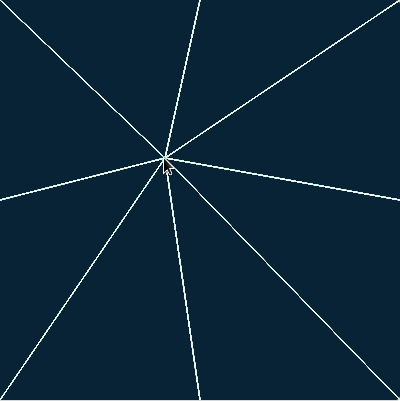
\includegraphics[width=0.40\textwidth]{illustrationer/kryds.png}
 \quad
 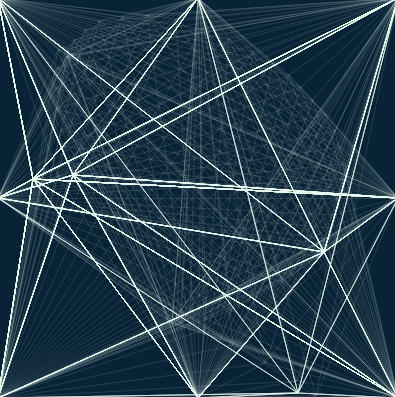
\includegraphics[width=0.40\textwidth]{illustrationer/kryds-tegning.png}
\end{center}
Remember to save the project!
\end{exercisebox}
